\documentclass[../main.tex]{subfiles}

Kommen wir nun zum Herzstück der Seminararbeit: Das Infrarotspektrometer. Es handelt sich um ein Werkzeug der Spektroskopie, das mithilfe der Absorptionseigenschaften der Elemente am Infrarotlicht eigenschaften von Substanzen nachweist.

\subsection{Komponenten}
\subsubsection{Strahlquelle}
Zunächst benötigen wir eine Infrarot-Strahlquelle, welche die Substanz durchdringt und danach mit einem Detektor gemessen wird. Als Strahlquelle bietet sich ein Lötkolben an.
\begin{figure}[ht]
    \centering
    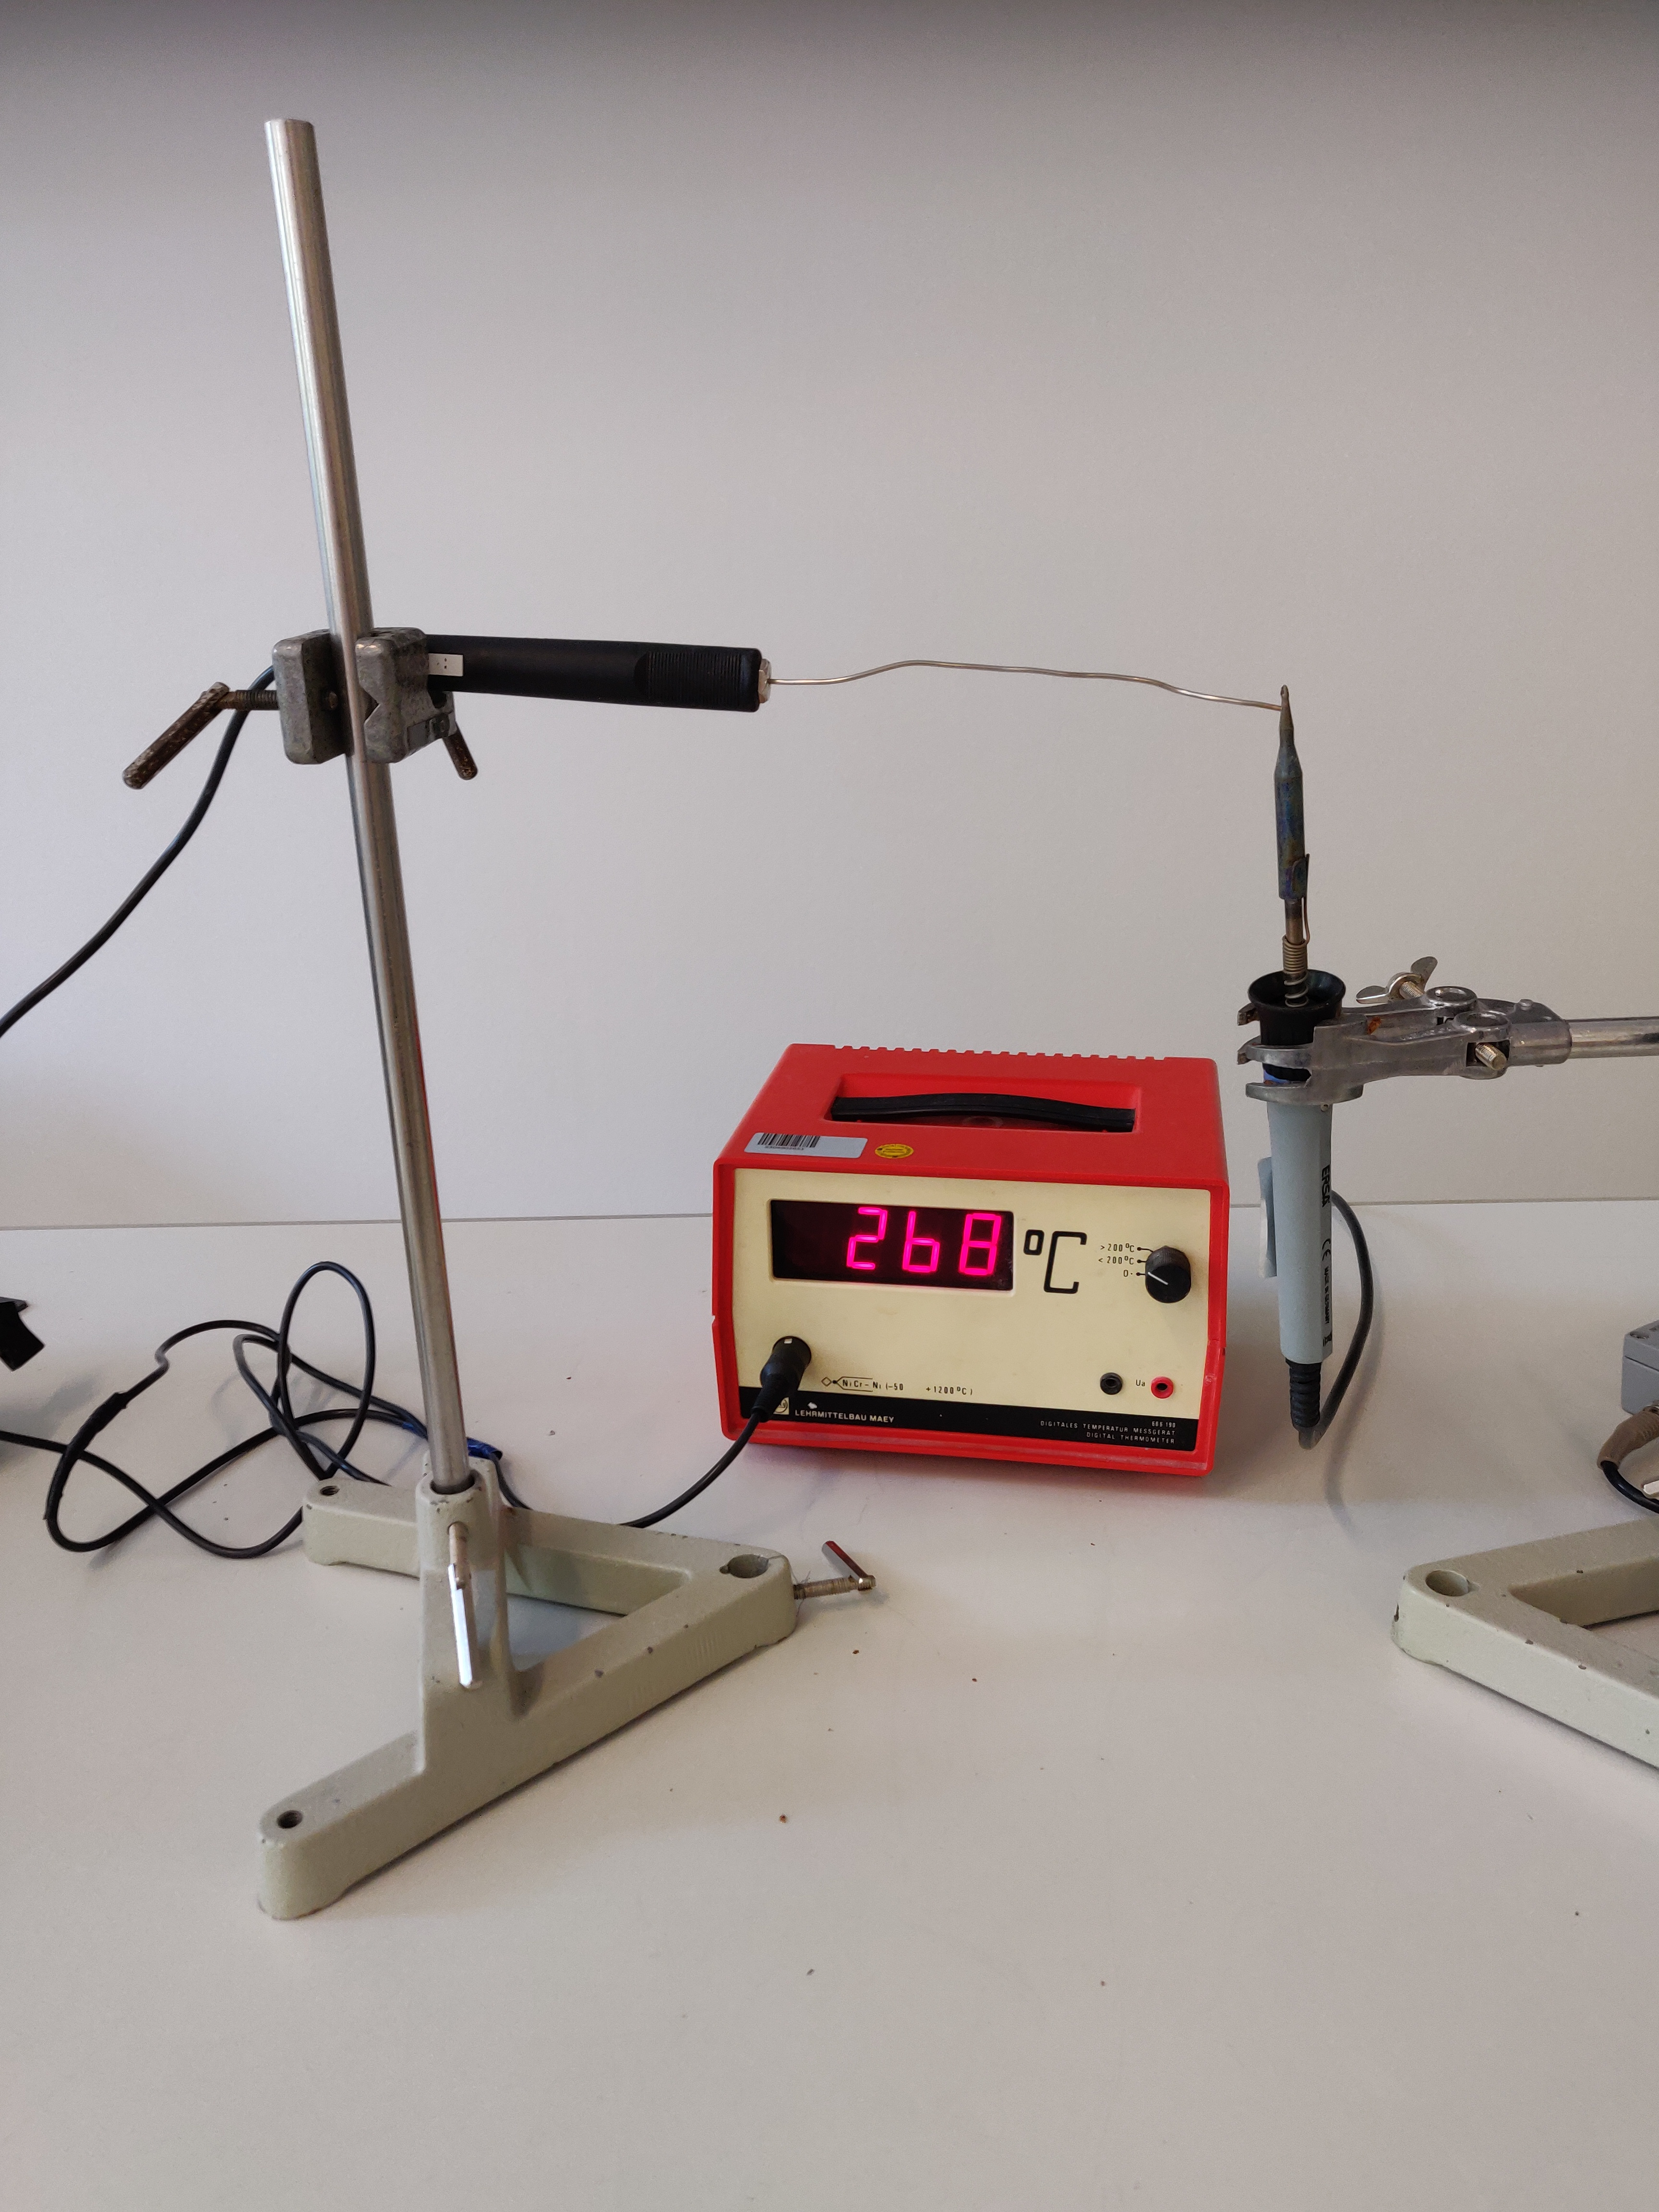
\includegraphics[width=0.2\textwidth]{experiment/11-loetkolben-temperatur.jpg}
    \caption{Lötkolben}
\end{figure}

% λ × T = b
% Lötkolben

\subsubsection{Abbildende Optik}
Um die Strahlung unseres Lötkolbens in eine Richtung zu fokusieren, müssen die nach außen gerichteten Wellen reflektiert werden. Ein Parabelförmiger Spiegel reflektiert die Strahlung so, dass sie in eine Richtung zeigt.
\begin{figure}[ht]
    \centering
    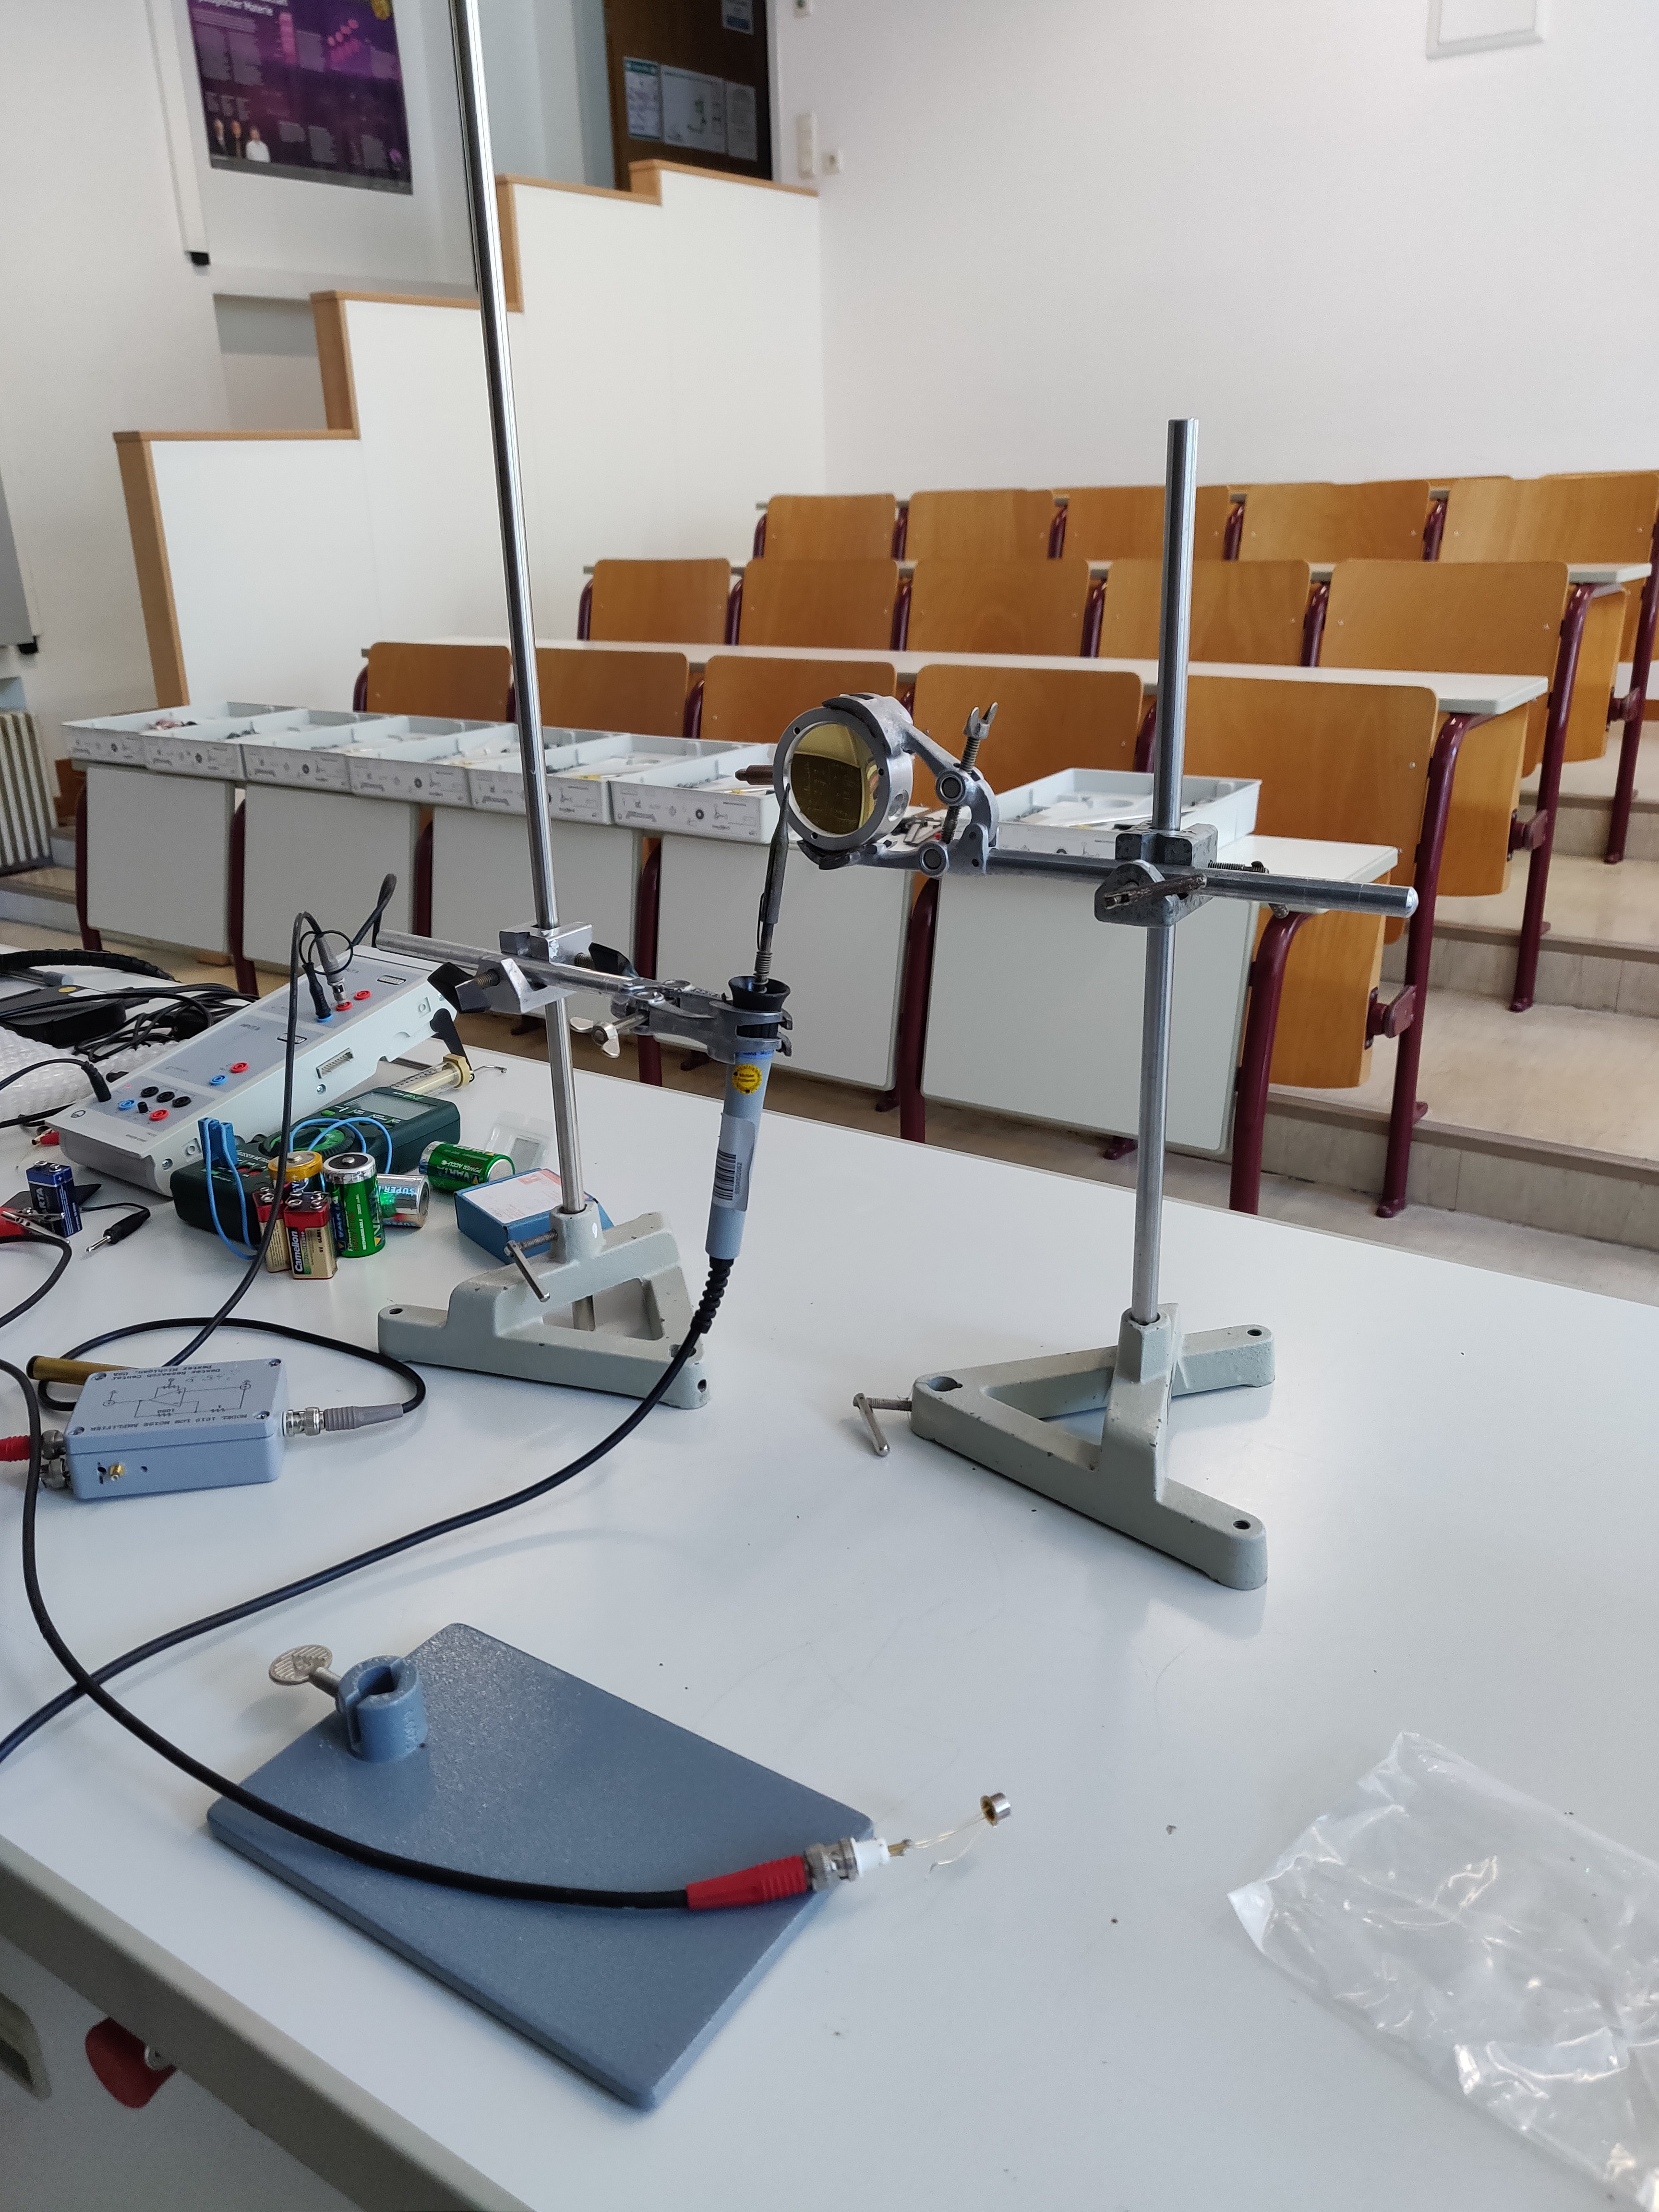
\includegraphics[width=0.2\textwidth]{experiment/13-loetkolben-spiegel.jpg}
    \caption{Lötkolben mit Spiegel}
\end{figure}

% Spiegel

\subsubsection{Optisches Gitter}
Das Gitter beugt die Strahlung in die verschiedenen Wellenlängen. Hierfür gibt es Gitter verschiedener Dichten, oder auch Reflexionsgitter, welche sowohl beugen als auch reflektieren.
\begin{figure}[ht]
    \centering
    \includegraphics[width=0.2\textwidth]{experiment/25-spektrometer-600-pro-mm.jpg}
    \caption{600 Linien / mm}
\end{figure}

% 600 Linien / mm
% Leypold
% Reflexionsgitter
